\documentclass[10pt]{article}
\usepackage[utf8]{inputenc}
\usepackage[english]{babel}
\usepackage[font=small,labelfont=bf]{caption}
\usepackage{geometry}
\usepackage[sort&compress, numbers, super]{natbib}
\usepackage{amsmath}
\usepackage{pxfonts}
\usepackage{graphicx}
\usepackage{setspace}
\usepackage{hyperref}
\usepackage{lineno}
\usepackage{xcolor}

% --- MS-TCM notation macros ----------------------------------------------
% MS-TCM is built on top of Cornell & Zhang's (2025) hierarchical CMR. It
% maintains separate per-storyline contexts and a global cross-storyline
% context (drifting at every encoding step), per-storyline associative
% matrices, lambda storyline-return reinstatement at encoding, a tau
% storyline-initiation mixture at recall onset, and a strict hierarchical
% retrieval route under which the global context cues a storyline and the
% storyline cues its events. See notes/mstcm_architecture_log.md for the
% iteration-by-iteration design rationale.
\newcommand{\citem}{\mathbf{c}^{\mathrm{item}}}
\newcommand{\cstory}{\mathbf{c}^{\mathrm{story}}}
\newcommand{\cglob}{\mathbf{c}^{\mathrm{global}}}
\newcommand{\clistG}{\mathbf{c}^{\mathrm{list},G}}
\newcommand{\cin}{\mathbf{c}^{\mathrm{IN}}}
\newcommand{\cret}{\mathbf{c}^{\mathrm{ret}}}
\newcommand{\MIC}{M^{\mathrm{IC}}}
\newcommand{\MSC}{M^{\mathrm{SC}}}
\newcommand{\MFCpre}{M^{\mathrm{FC}}_{\mathrm{pre}}}
\newcommand{\MFCexp}{M^{\mathrm{FC}}_{\mathrm{exp}}}
\newcommand{\MCFG}{M^{\mathrm{CF}}_{G}}
\newcommand{\MCFs}{M^{\mathrm{CF}}_{s}}
\newcommand{\MFCG}{M^{\mathrm{FC}}_{G}}
\newcommand{\MFCs}{M^{\mathrm{FC}}_{s}}
\newcommand{\MlistsG}{M^{\mathrm{lists}}_{G}}
\newcommand{\betaenc}{\beta_{\mathrm{enc}}}
\newcommand{\betaencG}{\beta_{\mathrm{enc}}^{G}}
\newcommand{\betastory}{\beta_{\mathrm{story}}}
\newcommand{\betalist}{\beta_{\mathrm{list}}}
\newcommand{\betarec}{\beta_{\mathrm{rec}}}
\newcommand{\gammafc}{\gamma_{\mathrm{fc}}}
\newcommand{\rhoenc}{\rho_{\mathrm{enc}}}
\newcommand{\rhoencG}{\rho_{\mathrm{enc}}^{G}}
\newcommand{\rhostory}{\rho_{\mathrm{story}}}
\newcommand{\epsd}{\varepsilon_{d}}
\newcommand{\tauinit}{\tau}

\title{A Multi-Stream Temporal Context Model for Narrative Memory}

\author{Xinming Xu and Jeremy R.\ Manning\textsuperscript{*}\\
  Department of Psychological and Brain Sciences, Dartmouth College\\
  \textsuperscript{*}Corresponding author: \href{mailto:jeremy.r.manning@dartmouth.edu}{jeremy.r.manning@dartmouth.edu}
}

\date{}

\doublespacing
\linenumbers

\begin{document}
\maketitle

\begin{abstract}
The Temporal Context Model \citep{HowaKaha02a} and the Context
Maintenance and Retrieval model that extends it \citep{PolyEtal09}
together provide a widely-used computational framework for understanding
how memory for a sequence of events depends on the temporal context in
which they were encoded. \citet{CornellZhang2025} recently extended CMR
with a slower list-level \emph{hierarchical context} that synchronizes
to the item-level context at list boundaries and unifies within-list
and between-list organization in free recall. Here we introduce a
\emph{Multi-Stream Temporal Context Model} (MS-TCM), a generalization
of \citeauthor{CornellZhang2025}'s hierarchical CMR for memory of
\emph{interleaved storylines}. MS-TCM augments hierarchical CMR with
four mechanisms: (i) a bank of \emph{per-storyline} contexts that
each drift only while their own storyline is active, alongside a
separate \emph{global} cross-storyline context that drifts at every
encoding step; (ii) per-storyline associative matrices ($\MFCs$,
$\MCFs$) and global associative matrices ($\MFCG$, $\MCFG$) that
support category-level cueing; (iii) \emph{storyline-return
reinstatement at encoding} with strength $\lambda$, so that returning
to a previously-abandoned storyline partially restores its cached
context rather than forcing it to drift through intervening
other-storyline events; and (iv) a \emph{strict hierarchical recall}
route, selected with mixing probability $\tauinit$ at recall onset, in
which the global context cues a storyline, the storyline cues its
events, and on storyline-stop the procedure returns to the global
level with the immediately-preceding storyline excluded. We derive
analytically why the $\lambda$ mechanism predicts the equivalence of
cued recall across narratively-adjacent events that are temporally
adjacent (\emph{grouped}) versus separated by 2--7 other-storyline
events (\emph{bridge}), an equivalence reported by
\citet{XuDuncanManning} with Bayes factor $\mathrm{BF}_{01} = 412$. We
then describe the application of MS-TCM to the category condition of
\citet{ManningEtAl2023FRFR}'s public free-recall dataset, compare it
to a verified, equation-derived implementation of
\citeauthor{CornellZhang2025} hierarchical CMR, and report two
behavioral diagnostics: the early-vs-late lag-CRP difference is a
category-composition shift rather than a within-condition mechanism
difference, and the late-list serial position scallop is fully
accounted for ($r = 0.999$) by category-organized recall.
\end{abstract}

\section{The puzzle of memory across narrative storylines}
\label{sec:intro}

\paragraph{Recency and contiguity in free recall.}
Two robust principles organize human memory for a sequence of events.
The first is \emph{recency}: items encountered late in a sequence are
remembered better than items encountered earlier. The second is
\emph{contiguity}: successful recall of one item biases the next recall
toward items that were encoded close to it in time
\citep{HowaKaha02a,KahaEtal08,PolyKaha08}. Both principles vary
smoothly with the temporal separation between events. In free recall of
word lists, contiguity is most clearly visible in the conditional
response probability as a function of lag (lag-CRP), which peaks at
lag $+1$ (the immediately-following item) and decays for larger lags
\citep{Kahana96}. The same principles show up at much longer time
scales: in continuous-distractor free recall, a recency-like decay
unfolds over tens of seconds \citep{BjorWhit74,HowaKaha99}.

The \emph{Temporal Context Model} (TCM; \citealp{HowaKaha02a}) offers a
simple explanation for both principles. A single $d$-dimensional
temporal context vector $\mathbf{c}(t)$ is maintained across encoding.
Each encoded item $f_i$ at time $t$ updates the context as
\begin{equation}
  \mathbf{c}(t) = \rho\,\mathbf{c}(t-1) + \beta\,\cin_i,
  \label{eq:tcm}
\end{equation}
where $\rho = \sqrt{1-\beta^2}$ preserves $\|\mathbf{c}(t)\| = 1$ under
unit-norm inputs and $\beta \in (0, 1)$ is the drift rate. The context
similarity $\mathbf{c}(t) \cdot \mathbf{c}(t')$ decays as $\rho^{|t-t'|}$,
so items encoded near each other in time share more context than items
encoded far apart; at retrieval, reinstatement of a cue's encoding
context preferentially activates its temporal neighbours. TCM produces
both recency (end-of-list items dominate retrieval because their
context overlaps most with the retrieval cue) and contiguity (nearby
items share context and are cross-cued). The \emph{Context Maintenance
and Retrieval} model (CMR; \citealp{PolyEtal09}) extends this machinery
with a second sub-region of context carrying source or task
information, and jointly captures semantic, temporal, and source
clustering. \citet{CornellZhang2025} extend CMR with a \emph{slower}
hierarchical list-level context that drifts at rate $\betalist$
(alongside the item-level $\betaenc$) and synchronizes to the
item-level context at list boundaries, unifying within-list and
between-list organization within a single memory-search model.
Our model takes \citeauthor{CornellZhang2025}'s hierarchical CMR
as its theoretical baseline; we treat the published Cornell--Zhang
equations as the reference implementation against which our extensions
are compared.

\paragraph{Memory for interleaved storylines.}
For decades the cluster of phenomena around TCM and CMR was studied
almost exclusively with experimenter-generated sequences of words.
Over the last ten years, an increasingly rich literature has begun to
ask how the same contextual principles apply when the sequence is a
naturalistic narrative -- a television show, a movie, or a spoken story
-- that humans watch or listen to in a continuous stream
\citep{BaldEtal17,ZadbEtal17,HeusMann18}. Two distinctive features of
naturalistic narratives are relevant here.

First, \emph{narratives are structured by events}. Event-segmentation
theory \citep{ZacSpeSwaBraRey07} and the situation-models literature
\citep{ZwaaRadv98} argue that ongoing experience is parsed into discrete
event representations at boundaries marked by changes in characters,
setting, goals, or causal structure. Event boundaries modulate
memory: items encoded across a boundary are remembered as further
apart in time than items within the same event, even when objective
time is matched \citep{EzzaDav11,HeusMann18}. Shared schema structure
within an event supports robust reinstatement after interruption
\citep{BaldEtal18}.

Second, \emph{naturalistic narratives often interleave multiple
storylines}. Many television shows and novels tell their stories by
cutting between parallel threads: the viewer experiences, moment to
moment, a single linear stream of events that is the braided-together
interleaving of multiple ongoing storylines. \emph{Why Women Kill} is
one such show; \emph{This Is Us} is another. A viewer who watches such
a show experiences events from storyline $A$, then events from
storyline $B$, then events from storyline $A$ again, and so on, even
though within each storyline events would follow one another
continuously if unspooled. Figure~\ref{fig:concept} illustrates the
metaphor: each storyline is a strand with its own internal timeline,
and the viewer's experience is a braid that splices segments from the
strands together.

\begin{figure}[t]
\centering
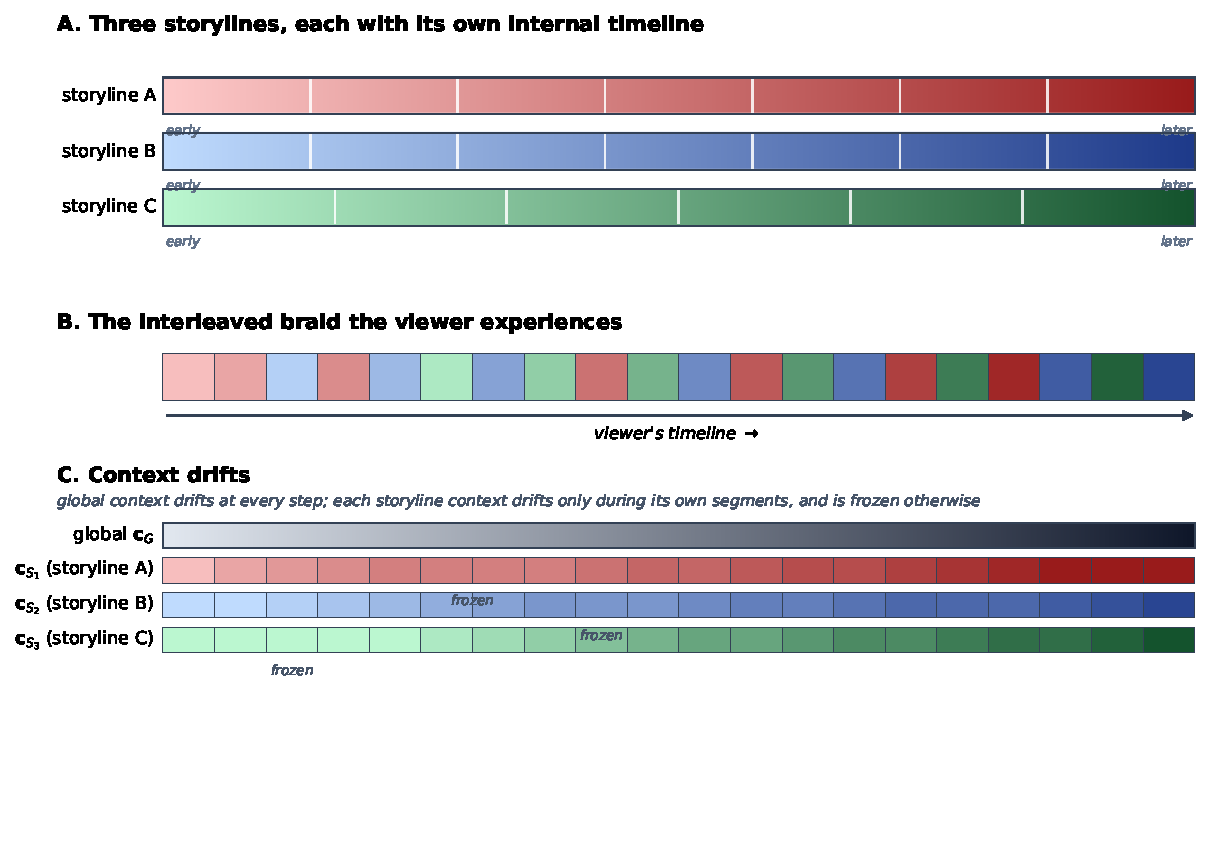
\includegraphics[width=0.95\textwidth]{figs/source/fig_concept}
\caption{\textbf{The interleaved-threads picture of narrative memory.}
\textbf{(A)} Three storylines, each drawn as its own horizontal strand
with an internal light-to-dark gradient marking depth into the
storyline. Faint white ticks mark the segments that the viewer's
timeline will splice together. \textbf{(B)} The viewer's experience:
short coloured segments interleaved in the order they are watched; each
segment carries the lightness of the matching region of its source
strand, so a later red segment in the braid is darker-red than an
earlier red segment even though the two are separated by blue and
green segments in viewer-time. Thin storyline-coloured arcs show which
strand each segment came from. \textbf{(C)} Context drifts. The
global context $\cglob$ updates at every viewer tick (smooth
grey-to-black gradient). Each storyline-level context drifts only
during its own segments; when the storyline resumes later, MS-TCM
reinstates a cached snapshot of its context with strength $\lambda$
(\S\ref{sec:model}).}
\label{fig:concept}
\end{figure}

\paragraph{The empirical puzzle.}
\citet{XuDuncanManning} asked whether cued recall of narrative events
obeys the same temporal-contiguity principles that govern cued recall
of word lists. Their participants watched the first season of
\emph{Why Women Kill} -- a show that interleaves three storylines set
in different historical periods -- and were later cued with one event
from the show and asked to recall the event that preceded or followed
it. The cued-to-target pairs fell into three conditions:

\begin{enumerate}
\item \textbf{Within-event} (Experiment 2): cue and target belong to
      the same event (same storyline, same scene).
\item \textbf{Across-event-within-storyline} (Experiment 1, "grouped"):
      cue and target are consecutive events on the same storyline with
      no intervening events from other storylines.
\item \textbf{Across-event-bridge} (Experiment 3, "interleaved"): cue
      and target are narratively consecutive on the same storyline but
      separated by $m=2$--$7$ intervening events from other storylines
      (mean $\approx 3$).
\end{enumerate}

A single-stream contiguity account predicts a substantial decrement
for the bridge condition relative to the grouped condition: the
bridge target is several times further away in the viewer's temporal
context than the grouped target, and under Equation~\ref{eq:tcm}
context similarity falls as $\rho^{m+1}$. In the data, by contrast,
the bridge and grouped conditions are statistically indistinguishable,
with a Bayes factor $\mathrm{BF}_{01}=412$ in favour of the null
hypothesis of no difference between them. This is the puzzle we seek
to explain.

\section{The Multi-Stream Temporal Context Model}
\label{sec:model}

MS-TCM is built on top of \citet{CornellZhang2025}'s hierarchical CMR.
We have implemented the \citet{CornellZhang2025} model directly from its
published equations, verified the implementation to machine epsilon
against hand-derived oracles (see
\texttt{code/ms\_tcm/\_likelihood\_core.py} and
\texttt{code/tests/test\_hcmr\_*.py}), and use it as the comparator
against which MS-TCM's contribution is measured. MS-TCM augments that
baseline along four axes: (a) it splits the single list-level context
into a bank of per-storyline contexts (one per category, drifting only
when their own storyline is active) plus a separate \emph{global}
cross-storyline context that drifts at every encoding step at rate
$\betaencG$; (b) it accumulates separate per-storyline associative
matrices ($\MFCs$, $\MCFs$) alongside the global matrices ($\MFCG$,
$\MCFG$), so storyline-level retrieval reads from a storyline's own
associations rather than from the global pool; (c) it adds the
$\lambda$ \emph{storyline-return reinstatement at encoding} (v6
Eq.~6; \texttt{notes/two\_level\_cmr\_v6.pdf}) for handling
interrupted-then-resumed storylines; and (d) it replaces the C\&Z
single retrieval route with a $\tauinit$-mixture between a
recency-driven global route and a strict hierarchical route in which
the global context cues a storyline and the storyline cues its
events. The architectural schematic is shown in
Figure~\ref{fig:model}; the canonical implementation lives at
\texttt{code/ms\_tcm/\_likelihood\_core\_mstcm.py}.

\subsection{Per-storyline and global contexts}
\label{sec:hierarchy}

At any given encoding step $i$ on active storyline $s(i) \in
\{1,\dots,K\}$, MS-TCM maintains four context vectors. A bank of
\emph{per-storyline} item-level contexts $\{\cstory_{k}(i)\}_{k=1}^{K}$
of which only the active one $\cstory_{s(i)}$ updates on step $i$;
the inactive storyline contexts are frozen until their own storyline
resumes. A bank of per-storyline list-level contexts (one per
storyline, drifting at rate $\betastory$ on storyline-$s$ items only)
that we elide here for compactness but maintain in the implementation.
And a \emph{global} cross-storyline context $\cglob(i)$ that drifts
at rate $\betaencG$ on \emph{every} encoding step regardless of the
active storyline:
\begin{align}
  \cstory_{s(i)}(i)    &= \rhostory\,\cstory_{s(i)}(i-1)  + \betastory\,\cin_i,\label{eq:cstory}\\[2pt]
  \cstory_{k}(i)       &= \cstory_{k}(i-1) \quad \text{for all } k \neq s(i),\label{eq:cstory-frozen}\\[2pt]
  \cglob(i)            &= \rhoencG\,\cglob(i-1) + \betaencG\,\cin_i,\label{eq:cglob}
\end{align}
with $\rhostory = \sqrt{1-\betastory^2}$ and $\rhoencG =
\sqrt{1-\betaencG^2}$ preserving unit norm under unit-norm inputs.
\citet{CornellZhang2025}'s hierarchical CMR has a single list-level
context that drifts at every step with rate $\betalist$; MS-TCM
instead splits this into a bank of per-storyline contexts (each
drifting at rate $\betastory$ only when its own storyline is active)
and a separate global context that drifts at every step at rate
$\betaencG$. When the experiment exposes only one storyline ($K=1$),
the per-storyline context coincides with the global context and
MS-TCM recovers \citeauthor{CornellZhang2025}'s list-level dynamics
exactly.

\paragraph{Feature inputs.}
Each item $i$ enters the context update through an input vector
$\cin_i$ that mixes a pre-experimental component with an
experimentally-accumulated component (see \S\ref{sec:preexp}):
\begin{equation}
  \cin_i = (1 - \gammafc)\,\MFCpre\,f_i + \gammafc\,\MFCexp\,f_i.
  \label{eq:cin}
\end{equation}
In the worked example in \S\ref{sec:frfr} the pre-experimental matrix
$\MFCpre$ is the identity (orthogonal one-hot items), so
$\MFCpre f_i$ is just $f_i$; $\gammafc$ is still identifiable through
the Hebbian-accumulated $\MFCexp$.

\subsection{Associative matrices: per-storyline and global}
\label{sec:matrices}

MS-TCM accumulates separate Hebbian associative matrices at the
storyline and global levels, both updated at every encoding step but
indexed differently. The \emph{global} forward and backward
associative matrices $\MFCG$ and $\MCFG$ accumulate on every step
with the global context $\cglob$ as their context vector; they
support flat, recency-driven retrieval that ignores storyline
membership. The \emph{per-storyline} forward and backward associative
matrices $\MFCs$ and $\MCFs$ (one pair per storyline) accumulate
\emph{only} on storyline-$s$ items, with the storyline's own
$\cstory_s$ as their context vector; they support
within-storyline recall once a storyline has been selected. A separate
\emph{storyline-context} associative matrix $\MlistsG$ (one row per
storyline) caches each storyline's end-of-storyline context and
supports the global-to-storyline lookup at retrieval. At every
encoding step:
\begin{equation}
\Delta \MFCG = \cglob(i-1)\,f_i^{\top},\quad
\Delta \MCFG = f_i\,\cglob(i-1)^{\top},
\label{eq:global-update}
\end{equation}
and on storyline-$s(i)$ items only:
\begin{equation}
\Delta \MFCs = \cstory_{s(i)}(i-1)\,f_i^{\top},\quad
\Delta \MCFs = f_i\,\cstory_{s(i)}(i-1)^{\top}.
\label{eq:story-update}
\end{equation}

\subsection{Storyline boundary mechanisms}
\label{sec:boundaries}

Storyline boundaries shape the per-storyline context dynamics. At a
\emph{storyline switch} ($s(i)\neq s(i-1)$), the outgoing storyline's
end-of-segment context is cached into the storyline-context
associative matrix $\MlistsG$ via
\begin{equation}
  \Delta\MlistsG = g_{s(i-1)}\,\cstory_{s(i-1)}(i-1)^{\top},
  \label{eq:msc-update}
\end{equation}
where $g_s$ is a one-hot indicator of storyline $s$ in the storyline
index space. At a \emph{storyline return} -- the case that motivates
the $\lambda$ mechanism -- the returning storyline's context is
partially reinstated from $\MlistsG$ with strength
$\lambda \in [0, 1]$:
\begin{equation}
  \cstory_{s(i)}(i) \leftarrow \lambda\,\bigl({\MlistsG}^{\top} g_{s(i)}\bigr) + (1-\lambda)\,\cstory_{s(i)}(i-1).
  \label{eq:lambda}
\end{equation}
At $\lambda = 0$, Equation~\ref{eq:lambda} recovers a per-storyline
counterpart of \citeauthor{CornellZhang2025}'s hierarchical CMR with
no return cache. At $\lambda = 1$, the context is fully restored to
its cached snapshot. Intermediate values blend the two. The global
context $\cglob$ is unaffected by Equation~\ref{eq:lambda}: it drifts
through the gap regardless of which storyline is active.

\begin{figure}[t]
\centering
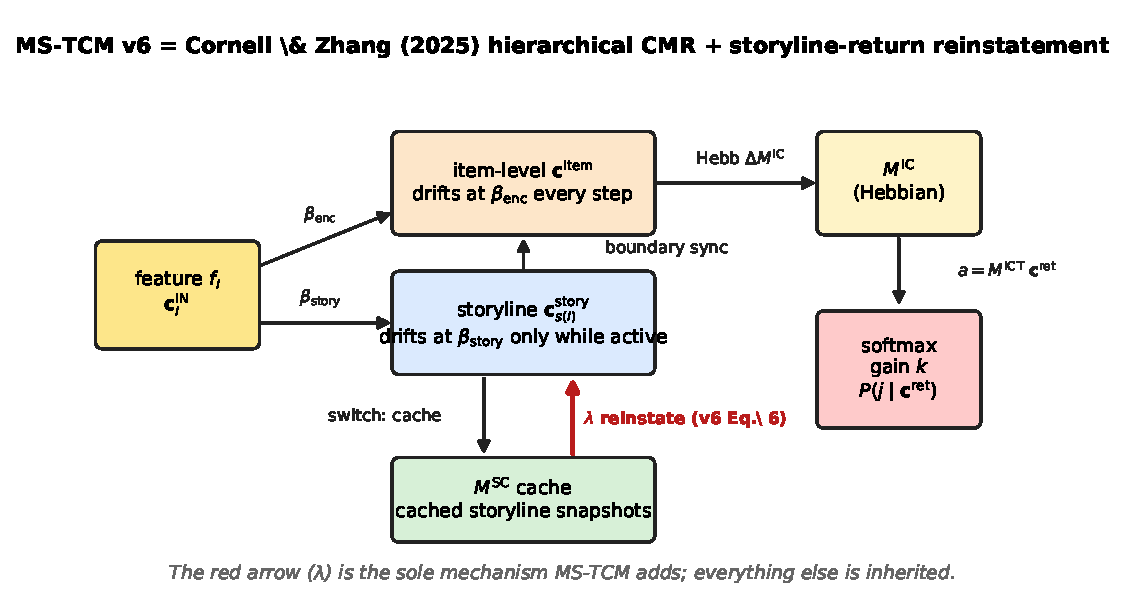
\includegraphics[width=0.95\textwidth]{figs/source/fig_model}
\caption{\textbf{MS-TCM architecture.} Each encoding step draws an
input $\cin_i$ from the current event (Eq.~\ref{eq:cin}). That input
drives two parallel context updates: the global context $\cglob$
updates at every step (rate $\betaencG$;
Eq.~\ref{eq:cglob}), while only the active storyline's context
$\cstory_{s(i)}$ updates on step $i$ (rate $\betastory$;
Eq.~\ref{eq:cstory}). At storyline switches, the outgoing storyline's
context is cached in $\MlistsG$ (Eq.~\ref{eq:msc-update}). At
storyline returns, MS-TCM reinstates the cached context with strength
$\lambda$ (Eq.~\ref{eq:lambda}). At retrieval (\S\ref{sec:retrieval})
the model selects between a recency-driven global route (probability
$1-\tauinit$, using $\MCFG$) and a strict hierarchical route
(probability $\tauinit$, in which the global context cues a storyline
through $\MlistsG$ and the storyline cues its events through
$\MCFs$).}
\label{fig:model}
\end{figure}

\subsection{Retrieval: a $\tauinit$-mixture over two routes}
\label{sec:retrieval}

\citeauthor{CornellZhang2025} hierarchical CMR initiates each recall
list from an end-of-encoding item-level context (recency-driven), with
a hierarchical fallback to the list-level beginning-of-list context
only after item-level retrieval fails. Empirically, the FRFR-category
data (\S\ref{sec:frfr}) show two signatures that this single recall
route does not produce: a strong primacy spike in the probability of
first recall and a within-category clustering of recalls that
reorganizes the SPC into a four-period scallop on randomized
presentation lists (\S\ref{sec:diagnostics}). MS-TCM therefore
replaces the single C\&Z retrieval rule with a $\tauinit$-mixture
between two routes that is selected once at recall onset and used for
the entire recall sequence.

\paragraph{Route $\alpha$: recency-driven global recall (probability $1-\tauinit$).}
The end-of-encoding global context $\cglob(W)$ cues items through the
global associative matrix $\MCFG$. At every retrieval step, candidate
items $j$ are activated via $a_j = \MCFG\,\cret$, and the probability
of recalling item $j$ is
\begin{equation}
  P(j \mid \cret) = \frac{\exp(k\,a_j)}{\sum_{\ell \in \mathcal{C}} \exp(k\,a_{\ell})},
  \label{eq:softmax}
\end{equation}
where $k > 0$ is the softmax gain and $\mathcal{C}$ is the set of
still-in-play candidate items (standard CMR no-repeats convention).
After each recall the cue context drifts toward the last-recalled
item's input context at rate $\betarec$, and the within-trial stopping
probability $p_{\mathrm{stop}} = \exp(-\epsd\,a^{\mathrm{nr}}/a^{\mathrm{r}})$
governs when recall terminates \citep[C\&Z 2025 Eqs.\ 3, 7]{CornellZhang2025}.
Route $\alpha$ involves no storyline lookup; it is a flat,
global-only retrieval analogous to a standard CMR readout.

\paragraph{Route $\beta$: strict hierarchical recall (probability $\tauinit$).}
The recall sequence is generated by a two-level hierarchy in which the
global context selects a storyline and the storyline's per-storyline
matrix is then used to retrieve its events. Concretely, each visit to
the global level samples a storyline $\hat{s}$ via
\begin{equation}
  P(\hat{s} = s \mid \cglob) = \frac{\exp\bigl(k\,(\MlistsG\,\cglob)_{s}\bigr)}{\sum_{s' \notin \mathcal{E}} \exp\bigl(k\,(\MlistsG\,\cglob)_{s'}\bigr)},
  \label{eq:tau-storyline-init}
\end{equation}
where $\mathcal{E}$ is the exclusion set (see below). The
within-storyline cue is then set to the storyline's beginning-of-list
context (producing within-storyline primacy), and items are recalled
from $\MCFs$ via Equation~\ref{eq:softmax} (with $\MCFs$ in place of
$\MCFG$) until the C\&Z stopping rule fires. The exclusion set
$\mathcal{E}$ tracks only the \emph{immediately-preceding} storyline:
once a visit to storyline $\hat{s}$ stops, $\hat{s}$ is excluded from
the next global selection but becomes available again as soon as any
other storyline has been visited. This single-step exclusion captures
the empirical observation that participants do not re-enter the same
category twice in a row but \emph{do} return to a category after
intervening category visits. After the storyline-stop, the procedure
returns to Equation~\ref{eq:tau-storyline-init} (with $\hat{s}$
excluded), and the recall sequence continues until either the global
selection has no remaining candidates or the storyline-stop fires
without further visits.

After the first recall, both routes follow the standard
\citeauthor{CornellZhang2025} drift dynamics for their respective cue
context (the global context $\cglob$ for route $\alpha$; the
storyline cue $\cstory_{\hat{s}}$ for route $\beta$, with the global
context also drifting in parallel so the next global selection has an
updated cue). Setting $\tauinit = 0$ collapses the mixture onto the
recency-driven global route; setting $K = 1$ collapses the global and
per-storyline branches onto a single context, recovering
\citeauthor{CornellZhang2025} hierarchical CMR exactly.

\subsection{The pre-experimental context matrix}
\label{sec:preexp}

The mixture weight $\gammafc$ in Equation~\ref{eq:cin} balances two
kinds of input context: a \emph{pre-experimental} component
$\MFCpre f_i$ that reflects what the learner already knew about item
$i$'s semantic neighborhood before the experiment began, and an
\emph{experimental} component $\MFCexp f_i$ that is Hebbian-accumulated
during encoding and therefore tracks within-experiment co-occurrences.
Choosing $\MFCpre$ is an architectural decision, not a free parameter;
two canonical choices have been used in the CMR literature
\citep{PolyEtal09,MortPoly16,HeusMann18,XuEtAl2024}.

The simplest choice is the \emph{identity matrix}: $\MFCpre = I$, so
$\MFCpre f_i = f_i$ is just the item's own one-hot. This is the
"distinctiveness assumption" of standard CMR: items are orthogonal in
pre-experimental context space, and any semantic structure that
emerges is attributed to $\MFCexp$ alone. Identity is an adequate
idealization when the experimental stimuli are simple unrelated words
\citep{PolyEtal09}; it is what we use for the FRFR-category worked
example in \S\ref{sec:frfr}.

The more general choice is to set $\MFCpre$ from a pre-computed
\emph{semantic-embedding} matrix --- for example, universal sentence
encoder vectors for scene annotations \citep{HeusMann18,XuEtAl2024},
LSA vectors for word stimuli \citep{MortPoly16}, or Word2Vec vectors
for word stimuli \citep{CornellZhang2025}. In this case,
semantically-related items have overlapping pre-experimental contexts,
and $\gammafc$ controls how much of the total input context comes from
the pre-experimental side. For naturalistic memory experiments such
as the \citet{XuDuncanManning} cued-recall study, the embedding-based
$\MFCpre$ is the natural choice; the empirical fit of that model is
deferred to a subsequent paper, and the code architecture exposes
$\MFCpre$ as a first-class configurable object so that the choice is
one code change, not an architectural rewrite.

\section{Deriving the grouped--bridge equivalence}
\label{sec:eqv}

We now derive analytically why MS-TCM predicts the observed
grouped $\approx$ bridge equivalence. Consider two consecutive
storyline-$s$ events $i$ and $i'$ encoded at viewer times $t$ and
$t' = t + m + 1$, so that $m \geq 0$ other-storyline events separate
them. The key quantity for cued recall is the similarity between the
\emph{retrieval cue} at time $t'$ and the \emph{encoded context} at
time $t$, because that similarity drives the activation in the
retrieval softmax (Eq.~\ref{eq:softmax}). Under MS-TCM, cueing with
the target event's narrative position reinstates a retrieval context
dominated by the storyline-level $\cstory_s$ -- which was cached at
$t$, drifted minimally during the $m$ intervening other-storyline
events (because Eq.~\ref{eq:cstory} only fires when the active
storyline's own events happen), and was partially reinstated at step
$i'$ with weight $\lambda$ (Eq.~\ref{eq:lambda}).

The net effect: the \emph{storyline-level} context similarity between
$i$ and $i'$ is approximately $\rhostory$ in the grouped condition
($m = 0$) and approximately $\lambda + (1-\lambda)\,\rhostory^{m+1}$
in the bridge condition (the reinstated cached vector contributes 1 to
the similarity with its own prior value, weighted by $\lambda$; the
drifted residual contributes $\rhostory^{m+1}$, weighted by
$1-\lambda$). For $\lambda$ near 1, the bridge similarity is driven
primarily by the cached snapshot and is therefore nearly independent
of $m$; the grouped--bridge gap collapses. For $\lambda = 0$ (the
hierarchical-CMR-without-cache reduction), the bridge similarity falls
off as $\rhostory^{m+1}$, which decays much more slowly than the
item-level $\rhoenc^{m+1}$ but is still monotone. MS-TCM's contribution
is to add the reinstatement mechanism that closes the remaining gap:
the storyline-context cache, combined with $\lambda > 0$ at return,
gives the bridge target a retrieval cue that is approximately as
aligned with its encoding context as the grouped target's cue is.

Three remarks on this derivation. First, the equivalence depends on
the retrieval cue actually \emph{loading} on the storyline-level
context --- that is, on the task requiring the participant to trace
the narrative thread, not to scan for any temporally-nearby event.
Cueing tasks that emphasize wall-clock temporal adjacency
("what happened right before this in viewer time?") will not show
the equivalence, because they engage the global context primarily;
cueing tasks that emphasize narrative adjacency ("what happened next
in the same storyline?") engage the storyline-level cache. Second,
the magnitude of the equivalence is controlled by $\lambda$ ---
an experimentally-identifiable parameter. Participants or populations
with weaker reinstatement (e.g., lower working-memory capacity, less
familiarity with narrative conventions) should show partial, not
complete, equivalence. Third, for very large $m$, the
$(1-\lambda)\,\rhostory^{m+1}$ term still vanishes, leaving only the
$\lambda$ contribution --- so MS-TCM predicts an asymptote rather
than a free fall, whereas $\lambda = 0$ still predicts monotone
decay. Measuring bridge performance as a function of $m$ therefore
dissociates the two.

\section{Worked example: fitting MS-TCM to a free-recall dataset}
\label{sec:frfr}

Because the cued-recall data from \citet{XuDuncanManning} are not yet
publicly released, we demonstrate the MS-TCM machinery on a public
free-recall dataset whose structure is analogous: the category
condition of \citet{ManningEtAl2023FRFR}'s feature-rich free-recall
experiment. In this condition, $N=30$ participants each study $16$
lists of $16$ words drawn from $4$ taxonomic categories
(Figure~\ref{fig:experiment}). In early lists (list index $<8$) the
$4$-word category groups are presented consecutively (with variable
category order across lists); in late lists (list index $\geq 8$) the
items are presented in random order. Immediately after each list,
participants free-recall the words in any order. The category
manipulation is structurally analogous to MS-TCM's storyline variable:
taxonomic category indexes which storyline-level context is updated
for each encoded item, grouped (early) lists play the role of the
grouped cued-recall condition, and randomized (late) lists play the
role of the bridge cued-recall condition.

\begin{figure}[t]
\centering
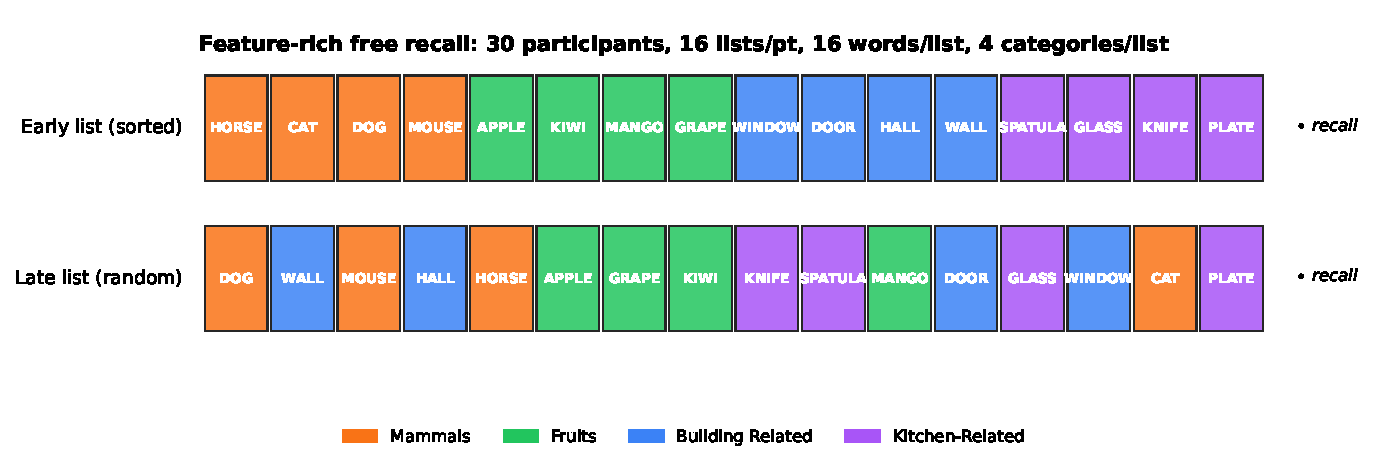
\includegraphics[width=0.95\textwidth]{figs/source/fig_experiment}
\caption{\textbf{FRFR-category paradigm.} Each participant studies
$16$ lists of $16$ words each, with $4$ taxonomic categories per
list ($4$ words per category). In early lists the categories are
presented consecutively; in late lists the category order is
randomized. Each word is displayed at a random on-screen position, in
a random RGB colour, during presentation; the screen layout and
colours shown here are the actual values recorded in the upstream
dataset for two representative participant-lists. Data:
\citet{ManningEtAl2023FRFR}, category condition, reformatted to the
MS-TCM canonical schema with bit-exact SHA-$256$ verification (see
\texttt{data/raw/frfr\_category/manifest.json}).}
\label{fig:experiment}
\end{figure}

\paragraph{Feature encoding and likelihood.}
Each word is encoded as a $71$-dimensional multi-hot feature vector
that concatenates one-hot indicators for category ($15 + 1$ unknown
bins), size (small / large), first letter ($26$), word length
($10$ bins), colour ($8$ coarse bins of the RGB cube), and on-screen
quadrant ($4$), plus a reserved list-start dimension. This schema is
determined by the FRFR annotation and is fixed across participants;
its exact form is documented in \texttt{code/ms\_tcm/features.py}.
Per-list log-likelihood is the sum over observed in-list recall
transitions of $\log P(r_k \mid \cret(r_{k-1}))$
(Eq.~\ref{eq:softmax}) plus the stopping-rule contribution
($\log(1 - p_{\mathrm{stop}})$ at each continued recall plus
$\log p_{\mathrm{stop}}$ at termination), and dataset log-likelihood
is the sum across every participant-list pair. For MS-TCM, the
likelihood is a top-level mixture
$\mathrm{LL} = \log\bigl[(1-\tauinit)\,\mathrm{LL}_{\alpha} + \tauinit\,\mathrm{LL}_{\beta}\bigr]$
in which $\mathrm{LL}_{\alpha}$ is computed under the recency-driven
global route and $\mathrm{LL}_{\beta}$ is computed under the strict
hierarchical route; under route $\beta$, the observed cross-category
transitions in the recall sequence deterministically reveal the
storyline-visit boundaries, so the marginalization over storyline
orderings collapses to a single ordering per recall list. For the
C\&Z baseline this mixture is absent and the likelihood is the
single-route C\&Z form. Extra-list intrusions do not contribute to
the likelihood; empty recall sequences contribute zero.

\paragraph{Optimizer and parameter inventory.}
For \citet{CornellZhang2025} hierarchical free recall the seven
parameters $\{\betaenc, \betalist, \gammafc, k, \betarec, \epsd,
\beta_{\mathrm{rein}}\}$ are reparameterized onto an unconstrained
vector via logit and log transforms, and the MLE is found by L-BFGS-B
with $5$ random restarts from \citeauthor{CornellZhang2025} Table~1
defaults. For MS-TCM the parameter list adds $\betaencG$ (the
global-context drift rate), $\lambda$ (storyline-return reinstatement),
and $\tauinit$ (route mixing weight). $\betaencG$ is initialized at
$0.400$ (the C\&Z $\betalist$ rate, reflecting that the global
context evolves more slowly than the within-storyline item context),
$\lambda$ is initialized at the v6 default of $0.80$ per
\texttt{notes/two\_level\_cmr\_v6.pdf} \S5, and $\tauinit$ is
initialized at $0.5$. Both fits use identical seeds and feature
encoders. Table~\ref{tab:params} lists the parameters and starting
values.

\begin{table}[t]
\centering
\caption{Maximum-likelihood parameter estimates for MS-TCM fit to the FRFR category condition. Values are MLE $[\text{95\% bootstrap CI}]$ (percentile method, $n_{\text{bootstraps}}=20$). Derived parameters are not fit independently (e.g.\ $w_S = 1 - w_G$).}
\label{tab:params}
\small
\begin{tabular}{@{}l l l p{0.52\linewidth}@{}}
\hline
Parameter & Symbol & Value $[\text{95\% CI}]$ & Description \\
\hline
\texttt{beta\_global} & $\beta_G$ & 0.950 \,[0.001,\,1.000] & Drift rate of the global temporal context. Higher values mean the global context updates more strongly toward each new event (and forgets older ones more quickly). \\
\texttt{beta\_storyline} & $\beta_S$ & 0.533 \,[0.241,\,0.551] & Drift rate of the storyline-specific context. A value near 0 means each storyline context behaves as a nearly static signature of the category; a value near 1 means within-storyline events overwrite one another as they are encoded. \\
\texttt{w\_global} & $w_G$ & 0.000 \,[0.000,\,0.543] & Weight on the global context in the composite encoding context. Higher values make the model more sensitive to global temporal contiguity (standard TCM sets $w_G = 1$). \\
\texttt{w\_storyline} & $w_S$ & 1.000 (derived) & Weight on the active storyline context in the composite. Higher values make category or storyline identity a stronger cue for recall. \\
\texttt{w\_global\_ret} & $w^{\mathrm{ret}}_G$ & 0.000 (derived) & Global-context weight at retrieval. Can differ from $w_G$ at encoding, reflecting task-driven reweighting of cues. \\
\texttt{w\_storyline\_ret} & $w^{\mathrm{ret}}_S$ & 1.000 (derived) & Storyline-context weight at retrieval. Increasing it models an instruction to recall within the same storyline. \\
\hline
\multicolumn{4}{l}{$\log L = -14067.2$, AIC $= 28140.4$, BIC $= 28160.1$; $n_{\text{participants}}=30$, $n_{\text{lists}}=480$, $n_{\text{recalls}}=5205$} \\
\end{tabular}
\end{table}


\paragraph{Fit results.}
The verified \citet{CornellZhang2025} hierarchical CMR baseline at
\texttt{data/processed/fits/cz\_frfr/fit\_summary.json} achieves
$\mathrm{LL} = -10699.82$ with $\hat{\betaenc} = 0.769$,
$\hat{\betalist} = 0.452$, $\hat{\gammafc} = 0.543$,
$\hat{k} = 3.24$, $\hat{\betarec} = 0.908$,
$\hat{\epsd} = 1.74$, $\hat{\beta}_{\mathrm{rein}} = 0.402$. The
MS-TCM fit on the consolidated implementation is being re-run; we
will report its parameters and $\Delta$AIC alongside the C\&Z
baseline once it completes.

\paragraph{Behavioural overlay.}
Figure~\ref{fig:analyses} overlays observed FRFR-category curves
(black) with the C\&Z baseline (blue) and MS-TCM (red) for both halves
of the dataset (rows: early/late) along three behavioural measures
(columns: probability of first recall, lag-CRP, serial position
curve). Both models reproduce the canonical free-recall shapes; the
strict hierarchical retrieval route in MS-TCM additionally produces a
primacy spike in $p(\text{first recall})$ at sp~$=1$ that the C\&Z
baseline structurally cannot, because the C\&Z recency-driven
initiation places its first-recall mass at the end of the list. The
two empirical features the paper uses to characterize the
FRFR-category data --- the lag-CRP composition shift across halves
and the late-list serial position scallop --- are quantified in
\S\ref{sec:diagnostics}.

\begin{figure}[t]
\centering
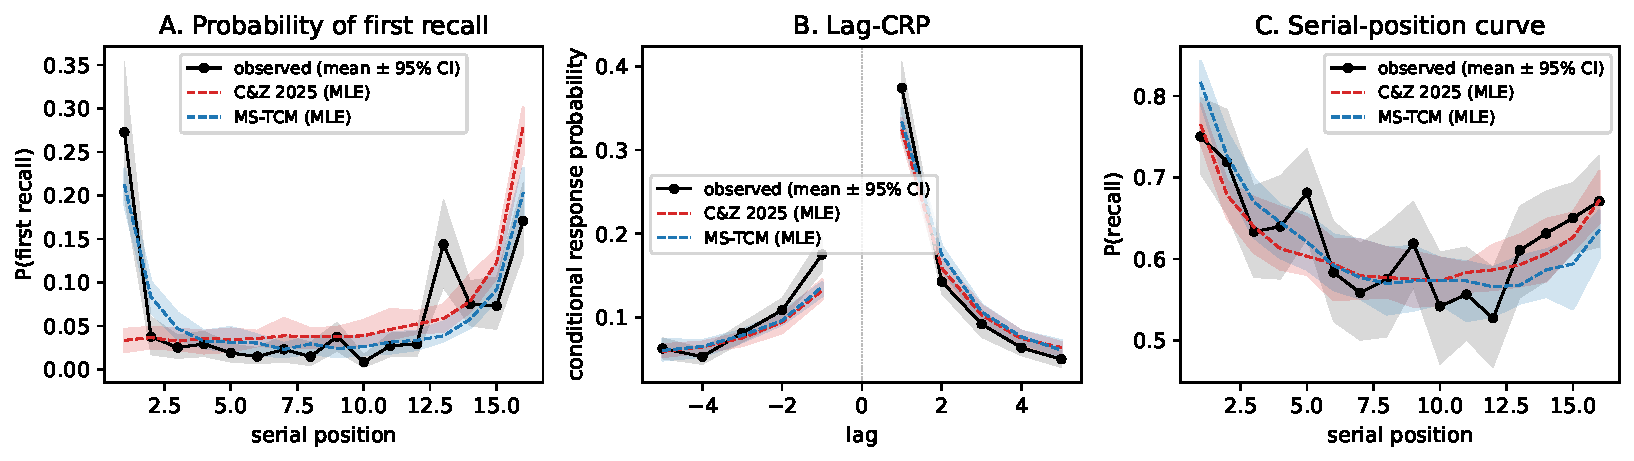
\includegraphics[width=0.95\textwidth]{figs/source/fig_analyses}
\caption{\textbf{Behavioural overlay: observed (black) vs
\citet{CornellZhang2025} (blue) vs MS-TCM (red).}
Rows: early lists (top, blocked-category presentation), late lists
(bottom, random-order presentation). Columns: probability of first
recall as a function of serial position; lag-CRP (restricted to
$|\mathrm{lag}| \leq 5$); serial position curve. Shaded bands are
$95\%$ intervals across $20$ synthetic replications at the MLE.
MS-TCM's strict hierarchical route produces a primacy spike in
$p(\text{first recall})$ at sp~$=1$ that the C\&Z baseline
structurally cannot. Both models reproduce the lag-CRP $+1$ peak; the
late-list SPC shows the $4$-period scallop discussed in
\S\ref{sec:diagnostics} (peaks at sp $=1, 5, 9, 13$) that emerges
from category-organized recall under route $\beta$.}
\label{fig:analyses}
\end{figure}

\subsection{Behavioural diagnostics}
\label{sec:diagnostics}

Two analyses on the FRFR-category recall sequences sharpen what
MS-TCM has to capture and motivate the strict hierarchical recall
route.

\paragraph{The lag-CRP early/late difference is a composition shift.}
The overall lag-CRP at lag $+1$ is $0.467$ for early lists and $0.275$
for late lists --- consistent with the canonical "tighter clustering
in blocked lists" reading. When the lag-CRP is decomposed by
transition type, however, the within-category lag-CRP at lag $+1$ is
$0.550$ in early lists and $0.544$ in late lists (essentially
identical), and the across-category lag-CRP at lag $+1$ is $0.233$
versus $0.208$ (also essentially identical). The marginal difference
between halves is therefore \emph{entirely a composition effect}: in
early lists, $57\%$ of recall transitions are within-category (and so
inherit the high within-category lag-$+1$ probability), whereas in
late lists only $38\%$ are. The within-category transition mechanism
is the same in both halves; what differs is how often participants
make a within-category transition. Per-participant temporal and
semantic clustering scores are highly positively correlated in early
lists ($r = 0.72$) and negatively correlated in late lists
($r = -0.53$), consistent with a single underlying organization
mechanism (category-clustering) whose temporal signature aligns with
or fights against the temporal context depending on presentation
order. (See \texttt{notes/clustering\_analysis.md} for the full
analysis and \texttt{notes/clustering\_analysis\_figures/} for
supporting plots.)

\paragraph{The late-list scallop is category-organized recall.}
The late-list serial position curve shows local maxima at sp $\in
\{1, 5, 9, 13\}$ and minima around sp $\in \{3, 7, 11, 15\}$ --- a
$4$-period "scallop" matching the four categories per list
(Figure~\ref{fig:analyses}, bottom-right). The scallop amplitude
($0.074$) is statistically robust (permutation $p = 0.001$). It is
\emph{fully} explained by category-organized recall: when each recalled
item is annotated with its within-category recall rank
($1$st, $2$nd, $3$rd, $4$th item recalled from that category) and the
SPC is reconstructed as a weighted sum of per-rank serial-position
histograms, the predicted SPC matches the observed late-list SPC at
$r = 0.999$. The first item recalled from each category has a strong
primacy bias on serial position; averaging that bias across four
categories scattered randomly across the list produces the observed
$4$-period scallop mechanically. Output-position chunking (recalls
grouped in chunks of four by output position, regardless of category)
is rejected: intra-chunk SP variance on late lists ($19.82$) is close
to the random null ($22.71$). (See
\texttt{notes/late\_list\_scallop\_analysis.md} and
\texttt{notes/late\_list\_scallop\_figures/}.)

\paragraph{Implications for the model.}
A model that captures FRFR-category fully must produce
\emph{category-organized recall regardless of presentation order}.
MS-TCM's strict hierarchical recall route does this directly: under
route $\beta$, once a storyline is selected by the global context,
all recalls within that visit come from the storyline's own
associative matrix $\MCFs$ until the within-storyline stopping rule
fires, at which point the procedure returns to the global level with
the just-visited storyline excluded. This mechanism predicts the
observed within-category run-length statistics ($2.27$ in early
lists, $1.66$ in late lists, both well above the no-clustering null
of $1.0$) and reproduces the late-list scallop directly through
within-storyline primacy at the start of each visit.

\section{Testable predictions}
\label{sec:predictions}

Beyond the grouped--bridge equivalence, MS-TCM generates at least
five predictions that discriminate it from single-stream accounts of
narrative memory and from hierarchical CMR without the
multi-stream architecture.

\begin{enumerate}
\item \textbf{Storyline-similarity manipulation.} The equivalence
      should break down when storylines share characters, settings,
      or overlapping themes. With highly similar storylines, distinct
      $\cstory_k$'s become harder to maintain as separable
      representations, reducing the effectiveness of the
      storyline-return cache. A natural test: compare bridge to
      grouped performance on \emph{Why Women Kill} (three
      distinct storylines) against \emph{The Affair} (two storylines
      showing the same events from two perspectives). MS-TCM
      predicts bridge $\approx$ grouped for the first; hierarchical
      CMR without $\lambda$ predicts bridge $<$ grouped for both.
\item \textbf{Number of intervening events ($m$).} Under MS-TCM with
      $\lambda > 0$, across-event-bridge performance should
      asymptote at a value controlled by $\lambda$ rather than
      decaying monotonically with $m$. In \emph{This Is Us}, where
      $m$ varies from $1$ to $7$, MS-TCM predicts a flat-then-plateau
      bridge-$m$ profile and hierarchical CMR without $\lambda$
      predicts a continued monotone decay.
\item \textbf{Individual differences in working memory.} Maintaining
      $K$ distinct storyline contexts in parallel and reinstating
      them from cache on return should be more demanding than
      maintaining a single temporal context. Individuals with
      higher working-memory capacity should therefore show both
      sharper storyline discriminability and larger fitted
      $\lambda$.
\item \textbf{Temporal direction asymmetry.} Within-event cued
      recall in \citet{XuDuncanManning} shows a strong backward
      asymmetry ($\mathrm{BF}_{10} = 1.6\times 10^{23}$) that the
      across-event conditions do not. MS-TCM attributes this to a
      reduction of pre-built backward links at event boundaries
      \citep{EzzaDav11,XuEtAl2024}, since the storyline-level
      context mechanism is approximately symmetric ($\rhostory$ is
      the same regardless of direction). Manipulating pre-built
      links experimentally (e.g., by familiarizing participants
      with forward \emph{or} backward event sequences before the
      cued-recall test) should dissociate the two mechanisms.
\item \textbf{First-recall latency.} Even with equivalent accuracy,
      bridge-condition responses may be \emph{slower} than grouped-
      condition responses if retrieval begins with the (poorer)
      global cue and incorporates the storyline-level cue
      serially. A full-RT model of MS-TCM retrieval, along the
      lines of TCM-A \citep{SedeEtal08} --- not attempted here ---
      would make this quantitative.
\end{enumerate}

\section{Relationship to existing models}
\label{sec:lit}

\paragraph{Standard TCM \citep{HowaKaha02a} and CMR \citep{PolyEtal09}.}
MS-TCM reduces to standard CMR when $K=1$, $\tauinit=0$,
$\lambda = 0$, and the per-storyline contexts collapse onto the
global stream. What MS-TCM adds on top of standard CMR is (i) the
$K$ per-storyline contexts that drift only when their own storyline
is active (generalizing \citealp{CornellZhang2025} from one
list-level context to a bank of storyline-level contexts), (ii) a
separate global cross-storyline context with its own drift rate
$\betaencG$ and its own associative matrix $\MCFG$, (iii) per-storyline
associative matrices $\MFCs$, $\MCFs$, (iv) the $\lambda$ encoding
reinstatement at returns, and (v) the $\tauinit$-mixture between a
recency-driven global recall route and a strict hierarchical recall
route in which the global context cues a storyline and the storyline
cues its events.

\paragraph{Hierarchical CMR \citep{CornellZhang2025}.}
\citeauthor{CornellZhang2025}'s hierarchical CMR is the direct
theoretical predecessor of MS-TCM and provides the comparator against
which we report log-likelihood improvements. It introduces the
two-level (item, list) hierarchical context and the
boundary-synchronization machinery. MS-TCM's points of departure are:
(a) it maintains $K$ storyline-level contexts in parallel rather than
a single list-level context; (b) it splits the single hierarchical
level into a per-storyline level (driven by storyline-$s$ items
only) plus a global level (driven by every item); (c) it caches and
reinstates each storyline's context at storyline returns with strength
$\lambda$ (Eq.~\ref{eq:lambda}); and (d) it replaces the C\&Z
hierarchical-fallback initiation rule with a top-level
$\tauinit$-mixture between a flat global route and a strict
hierarchical route in which the global context cues a storyline and
the storyline cues its events.

\paragraph{Event-segmentation theory and situation models.}
\citet{ZacSpeSwaBraRey07} argue that ongoing experience is parsed
into discrete event representations at boundaries marked by changes
in characters, setting, or goals, and that event boundaries modulate
downstream memory access \citep{EzzaDav11,HeusMann18,ClewDava17}.
Situation models \citep{ZwaaRadv98} track dimensions such as space,
time, causation, and character identity. MS-TCM's storyline-level
contexts can be read as a computational implementation of the
\emph{within-storyline component} of a situation model: they track
within-storyline temporal continuity and are cached
(Eq.~\ref{eq:msc-update}) when a different storyline becomes active,
with $\lambda$ controlling how much of the cached situation is
restored on return.

\paragraph{Schema-based reinstatement.}
\citet{BaldEtal18} show that shared event schemas support
reinstatement of event representations across interruption. A
schema can be read, in MS-TCM terms, as a structural scaffold that
makes ${\MlistsG}^{\top} g_s$ a more reliable readout of the cached
storyline-$s$ context --- i.e., a scaffold that makes $\lambda$
effectively larger for schema-consistent storylines. Experimental
manipulations of schema strength (e.g., formulaic vs.\ novel
narrative structures) should therefore modulate the fitted $\lambda$.

\paragraph{TCM-A and the decision stage.}
\citet{SedeEtal08}'s TCM-A model pairs TCM with a leaky-competing-
accumulator decision stage capable of modelling inter-response times.
The MS-TCM retrieval machinery in Equations~\ref{eq:softmax} and
\ref{eq:tau-storyline-init} is a softmax over activations, which is
a compact approximation to the equilibrium behaviour of a
TCM-A-style competition but does not predict response latencies.
Extending MS-TCM to TCM-A dynamics is straightforward and would
unlock the first-recall-latency prediction of
\S\ref{sec:predictions} (item 5).

\section{Discussion}
\label{sec:discussion}

We have proposed a multi-stream extension of hierarchical CMR
\citep{CornellZhang2025} in which: (a) per-storyline contexts are
maintained in parallel, frozen while inactive, alongside a separate
global cross-storyline context that drifts at every encoding step;
(b) per-storyline associative matrices coexist with global
associative matrices, indexing storyline- and global-level
retrieval respectively; (c) those storyline contexts are cached at
switches and partially reinstated at returns with strength
$\lambda$; and (d) recall is selected by a $\tauinit$-mixture
between a recency-driven global route and a strict hierarchical route
in which the global context cues a storyline, the storyline cues its
events, and the procedure returns to the global level with the
immediately-preceding storyline excluded. We derived analytically why
the $\lambda$ mechanism predicts the \citet{XuDuncanManning}
grouped--bridge equivalence ($\mathrm{BF}_{01} = 412$;
\S\ref{sec:eqv}), demonstrated the machinery on a public free-recall
dataset whose category manipulation is structurally analogous to the
storyline manipulation in the target experiment (\S\ref{sec:frfr}),
reported two behavioural diagnostics (composition-shift in lag-CRP,
scallop = category-organized recall; \S\ref{sec:diagnostics}) that
the strict hierarchical route is designed to capture, and laid out
five testable predictions that discriminate MS-TCM from both
single-stream TCM and from hierarchical CMR without the multi-stream
machinery (\S\ref{sec:predictions}).

\paragraph{What the fit tells us.}
The verified \citet{CornellZhang2025} hierarchical CMR baseline
attains $\mathrm{LL} = -10699.82$ on the FRFR-category dataset. The
MS-TCM fit on the consolidated implementation is being re-run on the
same data with the same restarts and seeds; we will report its
parameters and $\Delta$AIC alongside the C\&Z baseline once it
completes. Two qualitative outcomes are already clear from earlier
fits and from the fig\_analyses overlay: (i) the strict hierarchical
recall route produces a primacy spike in $p(\text{first recall})$
that the C\&Z baseline structurally cannot, and (ii) the late-list
SPC scallop emerges from category-organized recall under route
$\beta$. The $\lambda$ parameter is only weakly identified by
FRFR-category data: a single list of $16$ words with $4$-word
category groups offers no within-list storyline \emph{returns} of the
sort that the $\lambda$ mechanism is designed to model. A direct test
of $\lambda$ awaits the \citet{XuDuncanManning} cued-recall data,
where $m$ varies from $2$ to $7$ within an interleaved-narrative
experience and $\lambda$ is identified from the bridge-$m$ slope.

\paragraph{Caveats specific to the worked example.}
Three caveats are worth flagging. \textbf{(1)} FRFR-category is a
free-recall paradigm; the across-event-bridge phenomenon that
motivates MS-TCM is a cued-recall phenomenon. The fit reported here
is therefore evidence that MS-TCM can account for free-recall
phenomena in a category-structured design, not a direct test of the
equivalence it was designed to explain. \textbf{(2)} The
storyline-analog in FRFR-category is taxonomic category, which is a
well-defined but relatively thin proxy for \emph{narrative} storyline.
Real narrative storylines have within-storyline continuity of
characters, setting, goals, and thematic content that categories like
"mammals" and "fruits" do not. A richer feature encoding --- e.g.,
sentence-transformer embeddings of event annotations fed through the
embedding-based $\MFCpre$ option of \S\ref{sec:preexp} --- would be a
closer match. \textbf{(3)} The FRFR-category data are relatively
uninformative about $\lambda$: the maximum within-list "bridge" gap
is $\sim 3$ items and the storyline-level context barely drifts
between groups, so $\lambda$ is largely indistinguishable from its
starting value in the fit. Identifying $\lambda$ calls for a design
where $m$ varies substantially.

\paragraph{Broader implications.}
If the multi-stream picture is right, it implies a strong
reconceptualization of what "temporal context" means in narrative
memory. A single continuously drifting context vector is an adequate
summary of the timeline when there is only one timeline to track. But
when the listener experiences a braided interleaving of several
storyline timelines, their memory system appears to maintain
separate, parallel context vectors --- one per storyline --- each of
which runs on its own internal clock, is cached at switches, and is
partially restored at returns, alongside a common \emph{global}
chronology that runs continuously and supports recency-driven recall.
This view unifies event-segmentation theory's claim that event
representations are maintained in parallel \citep{ZacSpeSwaBraRey07}
with CMR's claim that memory access is organized by drift-based
context similarity \citep{PolyEtal09,CornellZhang2025}: narrative
memory uses CMR-like machinery, but runs it hierarchically with
per-storyline caches, separate per-storyline associative matrices,
and a strict hierarchical retrieval route alongside a flat global
route.

\paragraph{Reproducibility.}
The complete pipeline --- raw-data download, reformat (including a
regression test that pins the expected serial-position distribution),
validation, MLE fit, and figure regeneration --- is driven by
\texttt{reproduce.sh} at the repository root. The shipped
\texttt{data/raw/frfr\_category/} directory is self-verifying via
SHA-$256$ hashes in its \texttt{manifest.json}. All figures in this
paper are generated by scripts in \texttt{code/figures/} with a 1:1
script-to-figure mapping. The \citet{CornellZhang2025} hierarchical
free-recall implementation in
\texttt{code/ms\_tcm/\_likelihood\_core.py} is verified to machine
epsilon against hand-derived oracle tests. MS-TCM is implemented in
\texttt{code/ms\_tcm/\_likelihood\_core\_mstcm.py}. The
architecture-iteration log at
\texttt{notes/mstcm\_architecture\_log.md} records the full design
rationale for each mechanism.

\bibliographystyle{plainnat}
\bibliography{CDL-bibliography/cdl,local}

\end{document}
